\chapter{\fem}
\label{chp:fem}

In questo capitolo viene descritta l'azienda \textbf{\femsrl} in modo da contestualizzare i bisogni che hanno portato allo sviluppo della piattaforma web dedicata.

In particolare nelle sezioni \ref{sec:storia-fem} e \ref{sec:richieste} sono illustrate prima nascita ed espansione della spin-off, poi bisogni, richieste e necessità legate alla piattaforma sviluppata.

\section{La storia di \fem}
\label{sec:storia-fem}

\begin{wrapfigure}{r}{0.32\textwidth}
  \begin{center}
    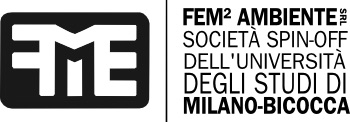
\includegraphics[width=0.3\textwidth]{images/logo-fem}
  \end{center}
\end{wrapfigure}

\textbf{\femsrl} è uno spin-off del Dipartimento di Biotecnologie e Bioscienze dell'Università degli Studi di Milano - Bicocca, nato con l'intenzione di creare prodotti e servizi per il largo pubblico finalizzati alla conoscenza e tutela della biodiversità. La mission è supportare i consumatori nelle scelte, rendendoli consapevoli sulla qualità delle risorse ambientali, e in questo modo fornendo gli strumenti necessari a migliorare il loro stile di vita, tutelando l'ambiente.

Ad inizio 2007 dall'incontro di Massimo Labra e Maurizio Casiraghi, due ricercatori del Dipartimento di Biotecnologie e Bioscienze dell'Università degli Studi di Milano Bicocca. Massimo Labra e Maurizio Casiraghi si occupano rispettivamente di tematiche botaniche e zoologiche, ma condividono, oltre a comuni tecniche di laboratorio, una simile visione della scienza. Principale collante delle diverse linee tematiche è la chiave di lettura evolutiva, alla luce della quale vengono analizzati e interpretati i risultati sperimentali.
Lo ZooPlantLab coniuga ricerca di base e applicata, in ambito zoologico e botanico. I principali progetti in corso prevedono l'utilizzo di un approccio molecolare. Tuttavia la formazione di molti membri del laboratorio ha previsto lavori di campo di zoologia e botanica, per cui l'integrazione delle nostre ricerche con l'approccio tradizionale è la norma. Inoltre, questa logica è la base delle numerose collaborazioni scientifiche vantate dallo ZooPlantLab. 

 Il logo dello ZooPLantLab è nato con l’idea di rappresentare due anime scientifiche, quella botanica e quella zoologica, che hanno deciso di condividere non soltanto un laboratorio ma un percorso di crescita scientifica senza barriere legati ai settore scientifici di origine
Per questa ragione nel logo la Z (zoologia) e la P (Plant –Botanica) non sono due lettere separate ma sono unite alla loro base, questo è il punto di partenza del gruppo.

Lo ZooPlantLab affronta quindi la diversità come ricchezza e momento di crescita. Troppo spesso sono state dedotte “teorie” su specie modello che si sono rilevate non adatte agli altri organismi. Pensiamo che solo integrando le nostre conoscenze, valutando il comportamento di animali e piante (ma anche batteri, funghi, ecc), analizzando la biodiversità nella sua totalità si possano produrre risultati scientifici più attendibili e applicabili al mondo reale.
Il logo dello ZooPlantLab è stato registrato alla Camera di Commercio di Milano nel 2009. La necessità di registrare è nata dalle applicazioni e i servizi che il gruppo fornisce a laboratori pubblici, privati e associazioni.
Lo ZooPlanLab è anche una sfida, un modo di cambiare la visione accademica della ricerca in cui troppo spesso si fissano paletti rigidi tra un settore scientifico e l’altro. Studenti, Dottorandi e phD dello ZooPlantLab non hanno barriere e questa è l’Università che vorremmo.


---

Fondato nel gennaio 2010 é cresciuto grazie al contributo e i risultati della ricerca di ZooPlantLab , il laboratorio di ricerca di zoologia, botanica e microbiologia nato qualche anno prima nello stesso dipartimento, che coniuga ricerca di base e applicata, in ambito zoologico e botanico. {\fem} é una piccola realtà con al centro i quattro soci fondatori:
\begin{itemize}
\item Dott. De Mattia Fabrizio, amministratore delegato e presidente di {\femsrl}. Scienziato dell’Ambiente e del Territorio, esperto in diagnostica molecolare vegetale, si occupa della gestione amministrativa e fiscale.
\item Dott. Ferri Emanuele, amministratore delegato. Biotecnologo specializzato nel settore bioinformatico e nelle analisi genomiche, é il responsabile della produzione e dei servizi di diagnostica molecolare.
\item Dott. Labra Massimo, socio fondatore. Biologo, ricercatore presso l’Università degli Studi di Milano - Bicocca e coordinatore dello ZooPlatLab; è il responsabile della ricerca e trasferimento tecnologico per la realizzazione dei prodotti. 
\item Dott. Casiraghi Maurizio, socio fondatore. Biologo, ricercatore e coordinatore dello ZooPlantLab; è il responsabile scientifico per la realizzazione e sviluppo dei servizi, responsabile delle relazioni internazionali e dei rapporti con l’Università.
\end{itemize}

{\fem} dispone di moderni laboratori ospitati presso l’Università, nei quali vengono sviluppati e testati i nuovi prodotti, eseguite analisi su matrici ambientali (es: acqua, aria o alimenti), si svolgono analisi del DNA e vengono messe a punto metodiche innovative di caratterizzazione molecolare. Grazie ad essi oggi {\fem}, pur mantenendo le sue solide radici universitarie ed investendo nella ricerca, si è affermata anche come società commerciale e propone al mercato nazionale ed internazionale prodotti e servizi all'avanguardia nei settori dell'ambiente, del food e della diagnostica molecolare avanzata.

Negli ultimi anni è diventato leader di mercato nella \emph{diagnostica molecolare di avifauna} tramite PCR (analisi del DNA), ed é nata la necessita di sviluppare una piattaforma adatta per gestire tutte le fasi di analisi e vendita dei servizi.


\begin{comment}

Lo ZooPlantLab nasce all'inizio del 2007 dall'incontro di Massimo Labra e Maurizio Casiraghi, due ricercatori del Dipartimento di Biotecnologie e Bioscienze dell'Università degli Studi di Milano Bicocca. Massimo Labra e Maurizio Casiraghi si occupano rispettivamente di tematiche botaniche e zoologiche, ma condividono, oltre a comuni tecniche di laboratorio, una simile visione della scienza. Principale collante delle diverse linee tematiche è la chiave di lettura evolutiva, alla luce della quale vengono analizzati e interpretati i risultati sperimentali.
Lo ZooPlantLab coniuga ricerca di base e applicata, in ambito zoologico e botanico. I principali progetti in corso prevedono l'utilizzo di un approccio molecolare. Tuttavia la formazione di molti membri del laboratorio ha previsto lavori di campo di zoologia e botanica, per cui l'integrazione delle nostre ricerche con l'approccio tradizionale è la norma. Inoltre, questa logica è la base delle numerose collaborazioni scientifiche vantate dallo ZooPlantLab. 

 Il logo dello ZooPLantLab è nato con l’idea di rappresentare due anime scientifiche, quella botanica e quella zoologica, che hanno deciso di condividere non soltanto un laboratorio ma un percorso di crescita scientifica senza barriere legati ai settore scientifici di origine
Per questa ragione nel logo la Z (zoologia) e la P (Plant –Botanica) non sono due lettere separate ma sono unite alla loro base, questo è il punto di partenza del gruppo.

Lo ZooPlantLab affronta quindi la diversità come ricchezza e momento di crescita. Troppo spesso sono state dedotte “teorie” su specie modello che si sono rilevate non adatte agli altri organismi. Pensiamo che solo integrando le nostre conoscenze, valutando il comportamento di animali e piante (ma anche batteri, funghi, ecc), analizzando la biodiversità nella sua totalità si possano produrre risultati scientifici più attendibili e applicabili al mondo reale.
Il logo dello ZooPlantLab è stato registrato alla Camera di Commercio di Milano nel 2009. La necessità di registrare è nata dalle applicazioni e i servizi che il gruppo fornisce a laboratori pubblici, privati e associazioni.
Lo ZooPlanLab è anche una sfida, un modo di cambiare la visione accademica della ricerca in cui troppo spesso si fissano paletti rigidi tra un settore scientifico e l’altro. Studenti, Dottorandi e phD dello ZooPlantLab non hanno barriere e questa è l’Università che vorremmo.


---

Il portale della diagnostica molecolare dedicato all'avifauna offre servizi di \emph{sessaggio}, \emph{diagnosi patologie} e \emph{Dna barcoding} disponibili per chi detiene, alleva o rivende avifauna.
Determinare il sesso precocemente e con sicurezza consente a chi intende assortire delle coppie di scongiurare perdite economiche e di tempo dovute all'assortimento di coppie formate da due maschi o due femmine, impossibili quindi a riproduzione. 
Il sessaggio da uovo consente a chi alleva a mano di soddisfare le richieste del cliente senza il rischio di fornire un soggetto del sesso non richiesto dopo un lungo lavoro di imprinting.

PATOLOGIE
I più recenti dati statistici indicano che la prevalenza di APV (poliomavirus) e BFDV (circovirus) in Italia sono rispettivamente del 31 e 26 %, valori che possono aumentare di oltre il doppio in determinati canali di vendita e scambi.

IDENTIFICAZIONE
L’innovativo servizio di identificazione tramite DNA (DNA barcoding) consente di stabilire la specie di appartenenza di qualsiasi soggetto a partire da diverse tipologie di materiale biologico (ad es. gusci di uovo, sangue, penne, piume, ecc.).

---

Per rendere più fruibile il servizio di analisi al cliente finale si é reso necessario creare un portale dedicato, il portale della \emph{Diagnostica Molecolare} che offre servizi di \emph{sessaggio}, \emph{diagnosi patologie} e \emph{Dna barcoding} disponibili per chi detiene, alleva o rivende avifauna.

La relazione cerca di descrivere lo sviluppo dalla base di un portale di questo tipo, e sarà composta da -N- parti principali: 

---
\end{comment}


\section{Le richieste}
\label{sec:richieste}

